\chapter{Literature Review}
\label{litreview}

\section{Rasterisation rendering}
Modern graphical hardware is heavily specialised for the tasks involved in rasterisation. Rasterisation refers to the conversion of mathematically defined vector geometry to a raster image on screen.

There are two main operations involved in rendering using rasterisation: transformation, the act of converting geometry defined in 3D space to coordinates on the screen, taking into account perspective; and rasterisation itself, the act of converting this transformed vector geometry into a raster image for display. These operations, and the operations required to complete them, are the purpose for which modern graphics hardware is specialised.

\subsection{Transformation}
In graphics, the term transformation refers to the mathematical mapping of one set of coordinates to another. The main transformations involved in 3D rendering include translation, rotation, scaling, and projection. Translation is defined as a transformation which offsets a point by a certain amount in each axis, whereas rotation is a transformation which rotates a point around the origin by some angle in some axis. Scaling is a transformation which increases the distance from 0 in each axis by a multiplier.

\begin{figure}
	\centering
	\subfloat[Translation]{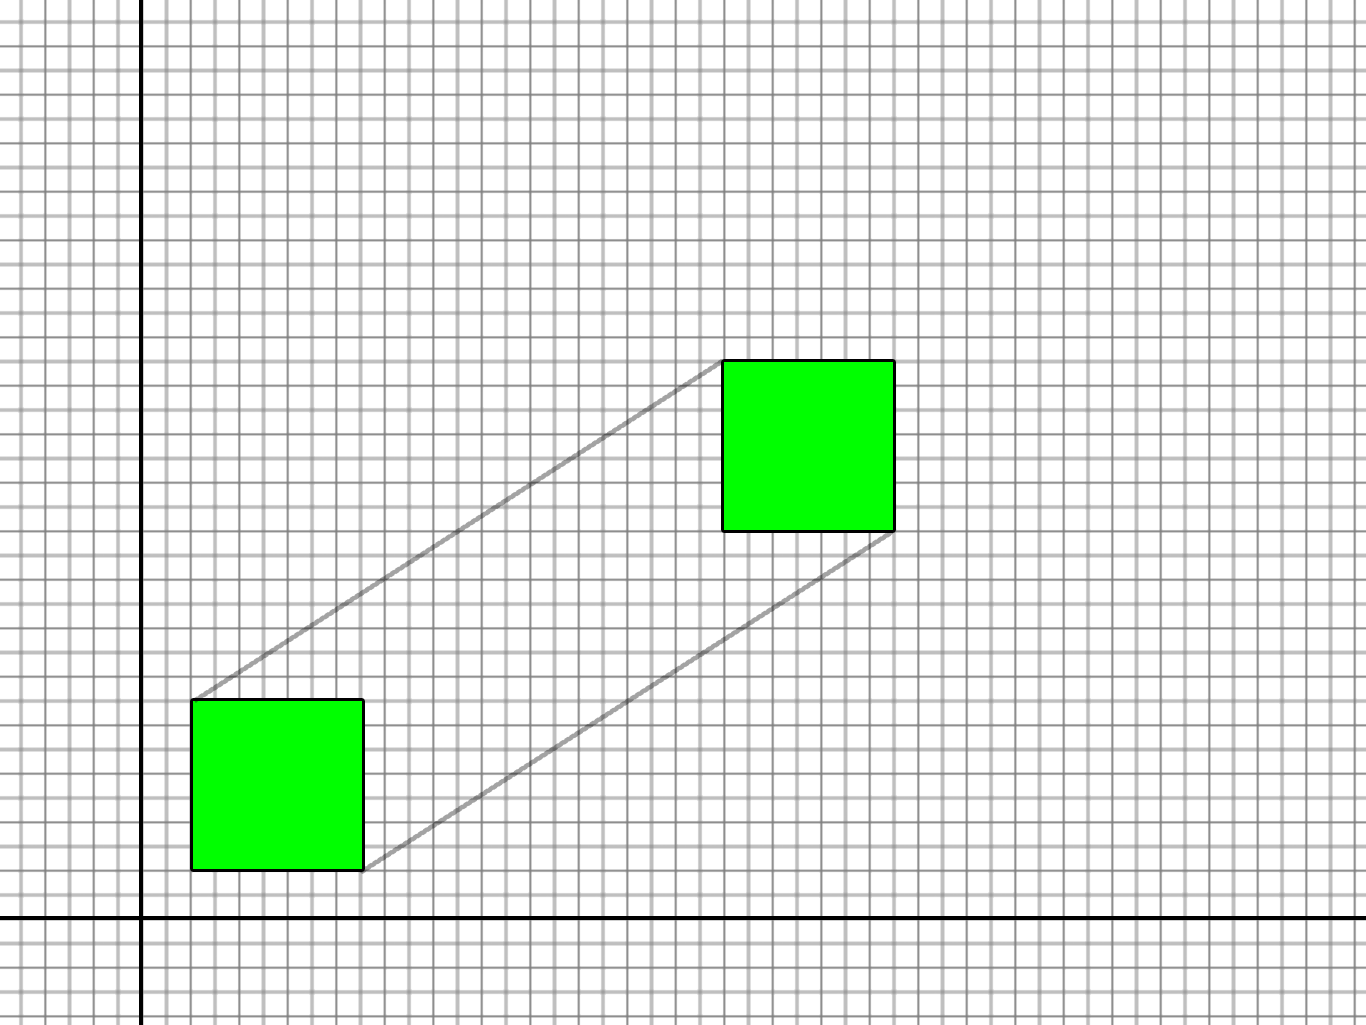
\includegraphics[width=2in]{translation.png}}
	~
	\subfloat[Rotation]{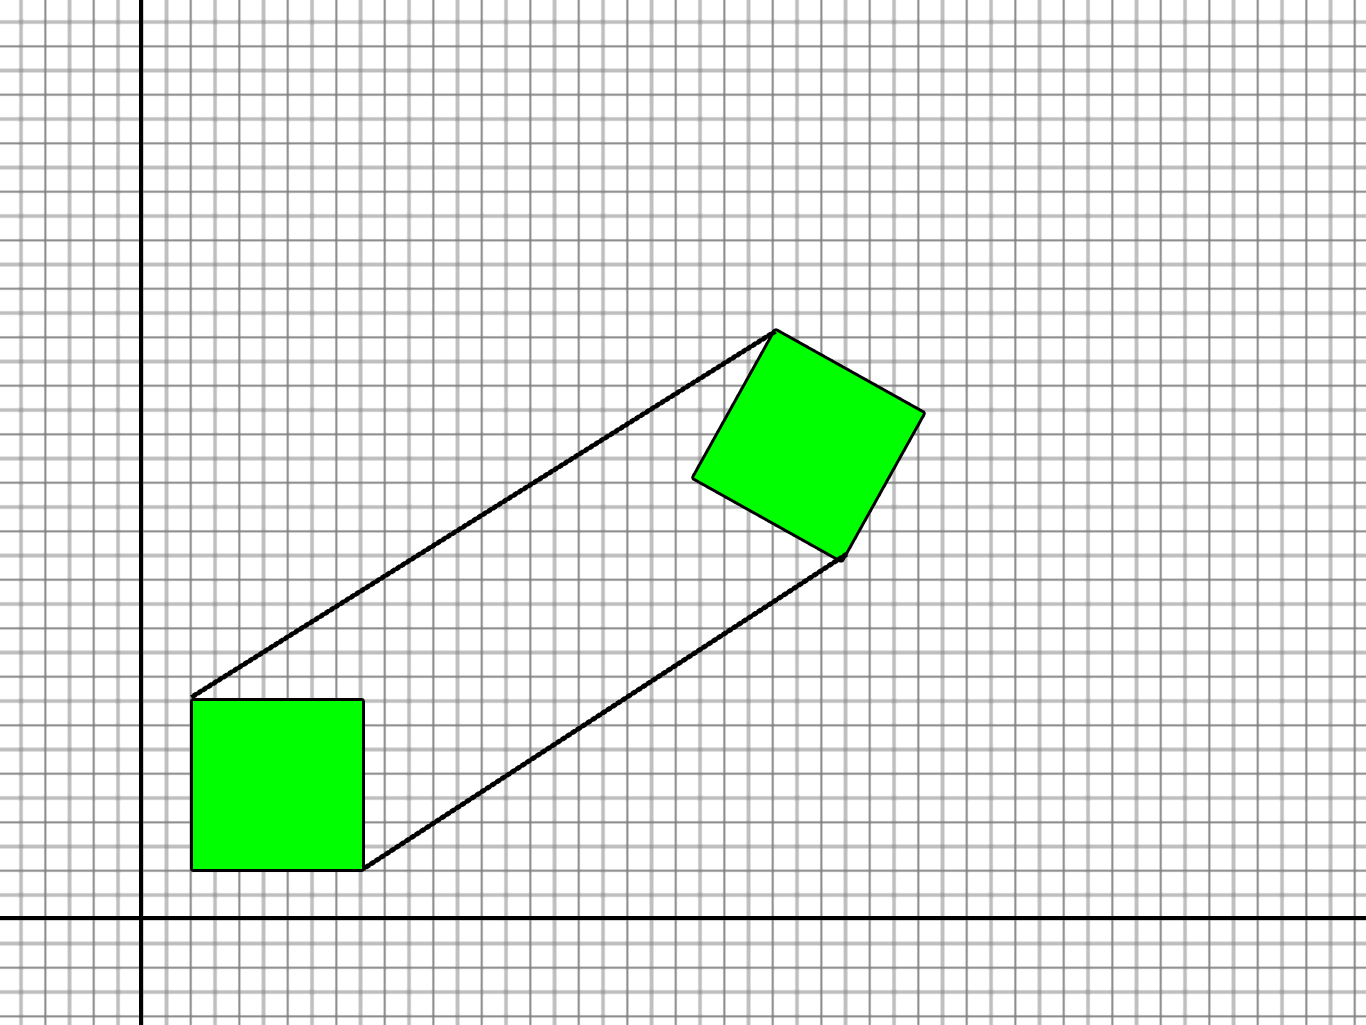
\includegraphics[width=2in]{rotation.png}}
	~
	\subfloat[Scaling]{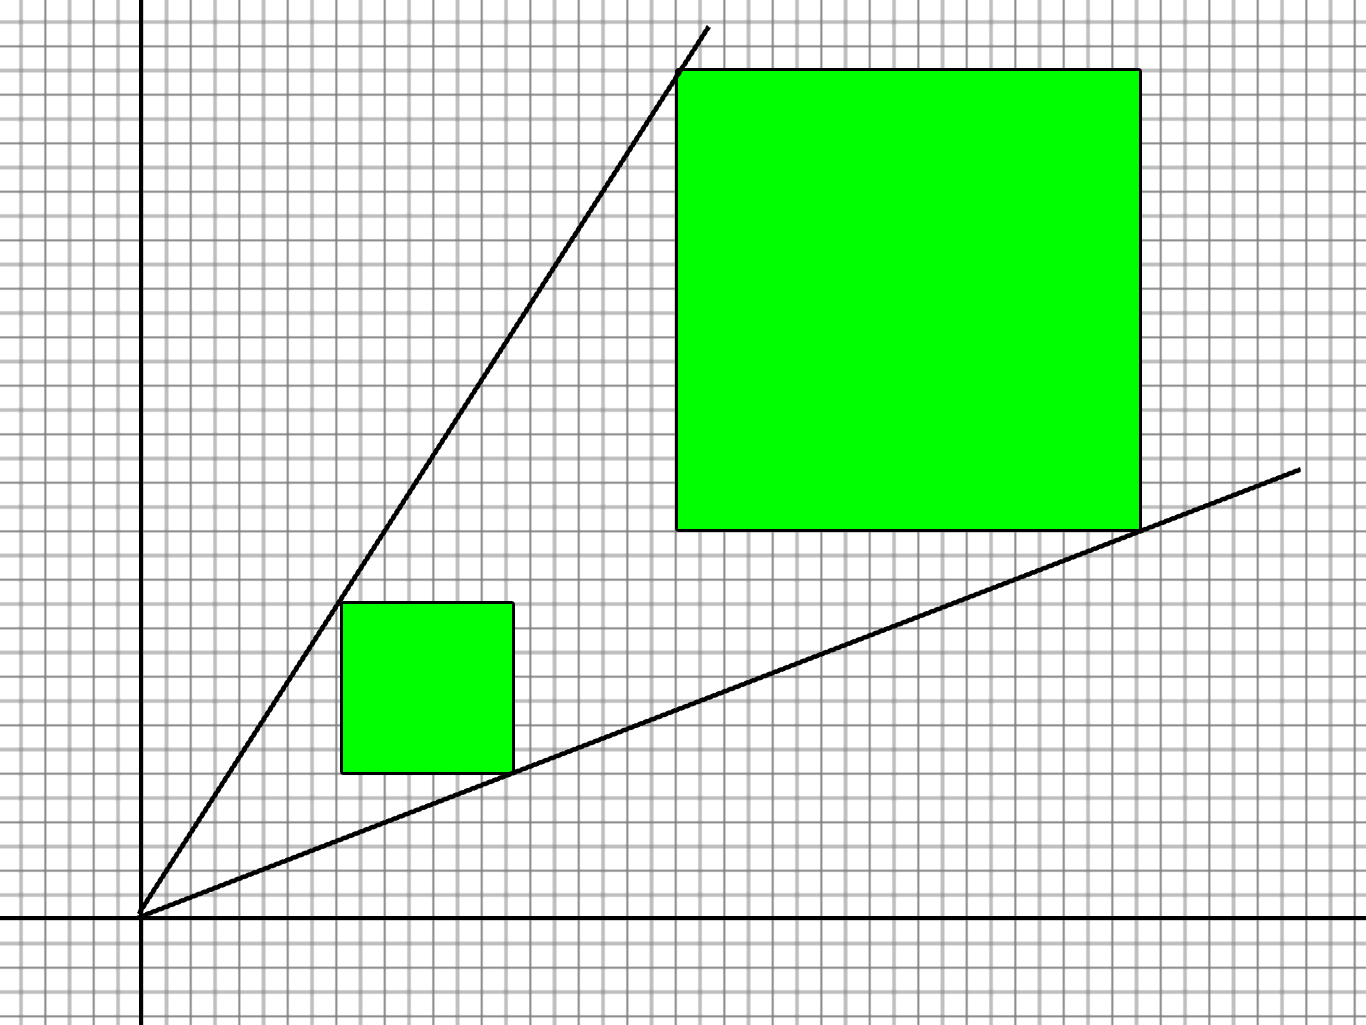
\includegraphics[width=2in]{scaling.png}}

	\caption{Geometric transformations}
	\label{fig:transformations}
\end{figure}

Projection is a transformation which describes the mapping of three-dimensional points onto a two-dimensional plane. In order to give the rendered image perspective, we use a perspective projection. A perspective transformation takes into account the field of view (FOV) of the viewer, as shown in figure \ref{fig:perspective-projection}, in order to provide a perspective-correct representation of the scene.

\begin{figure}
\centering
	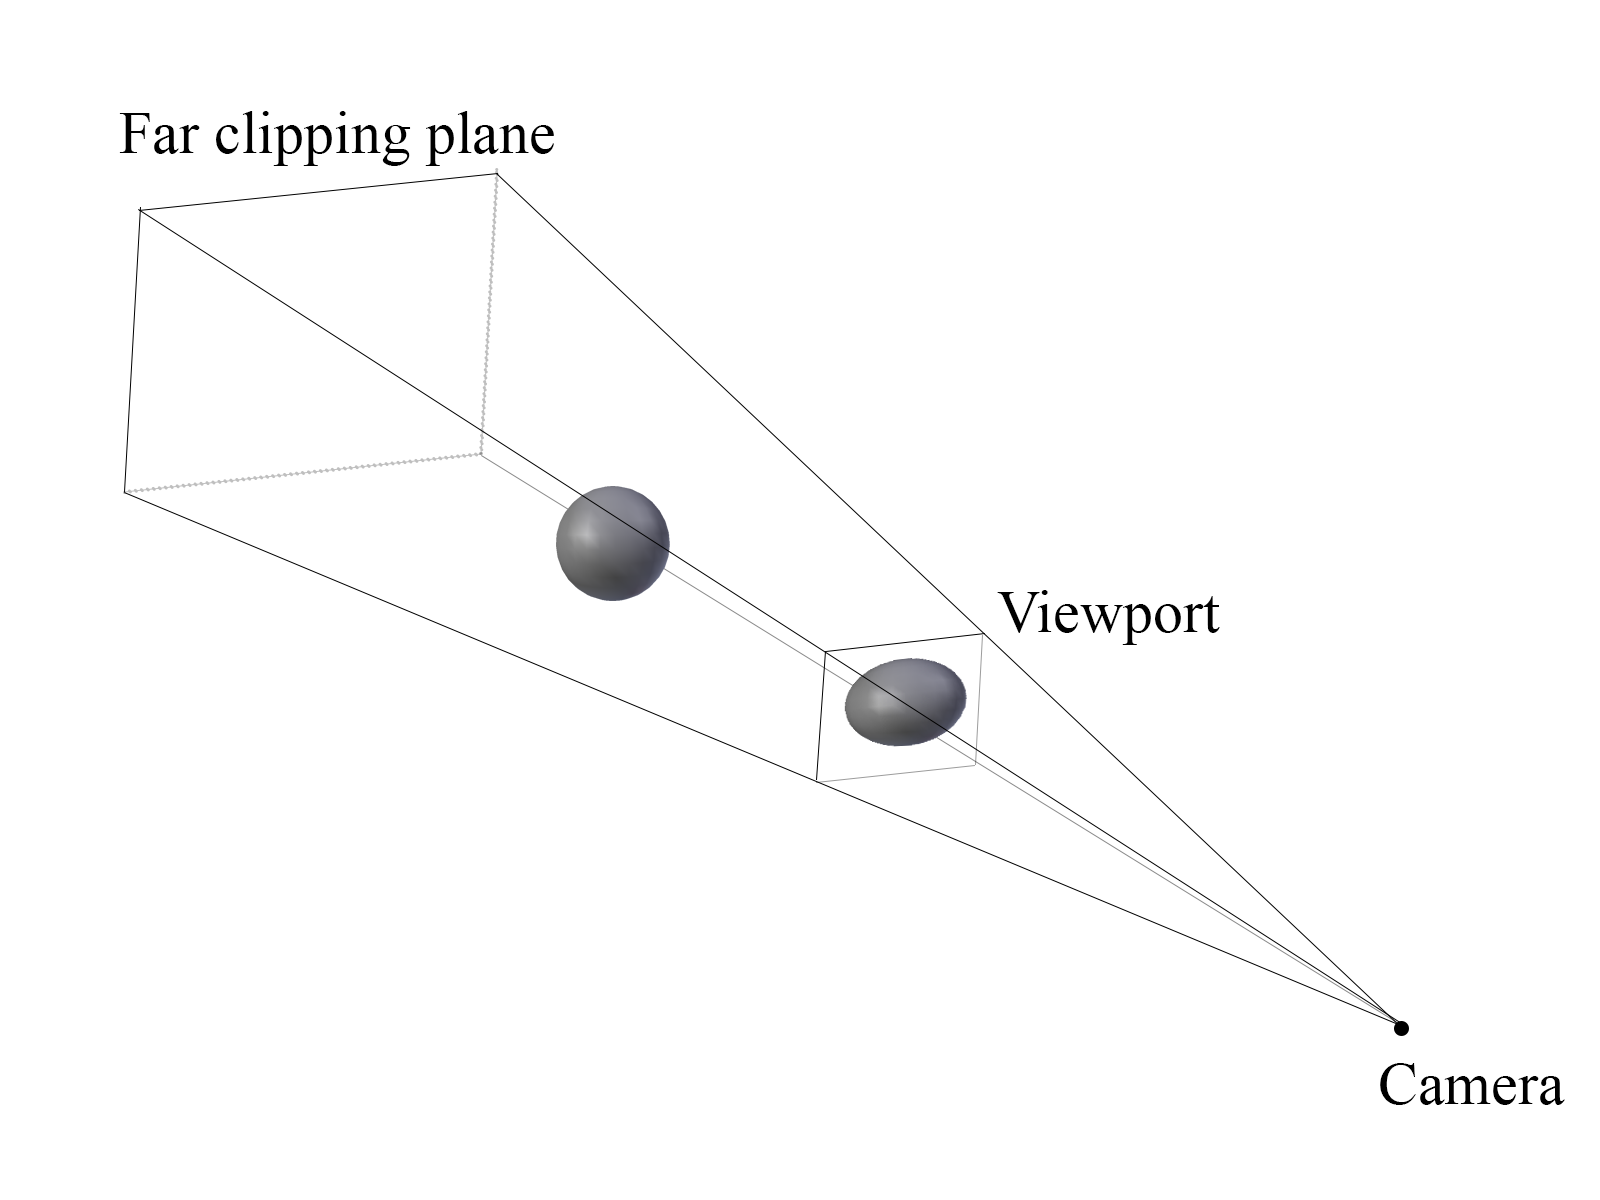
\includegraphics[width=14cm]{frustum.png}
	\caption{A perspective projection transformation}
	\label{fig:perspective-projection}
\end{figure}

In rasterisation rendering, we aim to take vector values defining the "world space" (position within the scene) coordinates of the geometry of the surfaces we are attempting to render and map them to the screen such that it produces a 2D image of the 3D scene.

In order to accomplish this, we consider three main transformations: perspective projection, which is defined by a projection transformation; the model transformation, which uses translation, rotation, and scale transformations in order to represent the object's position in the scene; and the view transformation, which uses a translation and a rotation transformation in order to represent the camera's position and rotation in the scene.

We use 4x4 matrices to represent these transformations, as this allows us to represent perspective projection and translation transformations (as well as the other required transformations.) As the matrices are square, an added advantage that they can be multiplied together to result in a combined transformation known as a model-view-projection (MVP) matrix.

This overall transformation defines the transformation of points from world space to a position on the viewport, in "viewport space". This normalised coordinate space, often from -1 to 1 on both axes, where -1 and 1 are the extremities of the field of view, must then be scaled to their final coordinates on the screen, in "screen space", based on the dimensions of the viewport. Vertices outside of this range are outside of the field of view of the projection.

This scaling can be described very simply. For a viewport space defined from -1 to 1 on both axes, where -1 represents the left and bottom of the viewport, and 1 represents the top and right of the viewport, this transformation can be done by adding 1 to both coordinates to get them in the range 0..2, dividing both coordinates by 2 to get them in the range 0..1, and multiplying by the dimensions of the viewport, to get the coordinates in screen space. This can be written algebraically as:

\begin{align}
	x_{screen} &= (1 + x_{viewport}) \cdot \frac{width_{viewport}}{2}
	\\
	y_{screen} &= (1 + y_{viewport}) \cdot \frac{height_{viewport}}{2}
\end{align}

In different rendering frameworks the definition of the viewport can vary, but the principles are the same. The basic transformations required to make this conversion are simply a 2D translation and scale.

\subsection{Rasterisation}
Once geometry has been transformed into screen space, the process of rasterising triangles in order to display them on the screen is incredibly simple (see section \ref{pct} on polygon scan conversion for one possible method.) However, this is not the only step which is required to produce a 2D representation of a 3D scene. The next problem is how we should colour each pixel in the rasterised triangle in order to make it look 3D. Once a pixel is determined to be inside the triangle, the pixel is then shaded in order to determine its final colour on the screen.

\subsubsection{Shading}
Shading refers the process of determining a colour for a pixel on the screen. With rasterisation-based rendering techniques, this colour is usually determined using attributes from the triangle. Estimations of a number of lighting effects are used in order to determine this colour. There are three main contributions normally taken into account with rasterisation-based rendering techniques: ambient reflection, diffuse reflection, and specular reflection.

\begin{figure}
	\centering
	\subfloat[Flat shading]{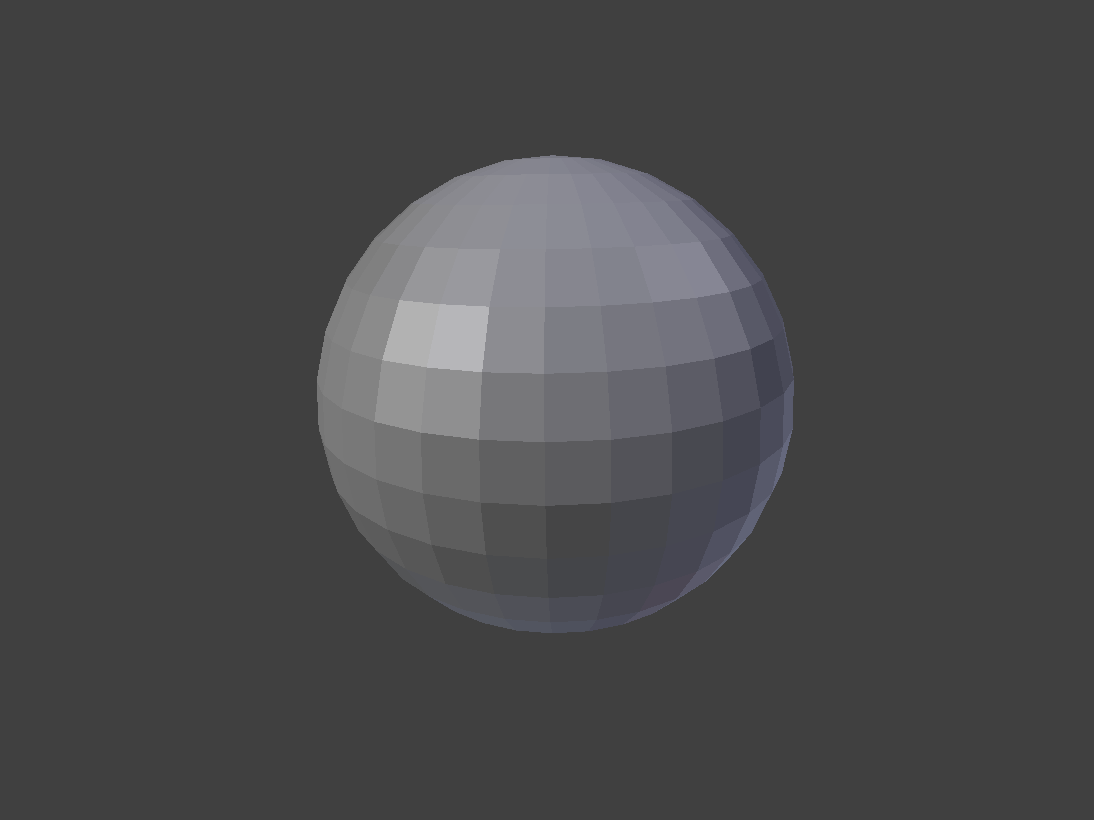
\includegraphics[width=3in]{flat_shading.png}}
	~
	\subfloat[Smooth shading]{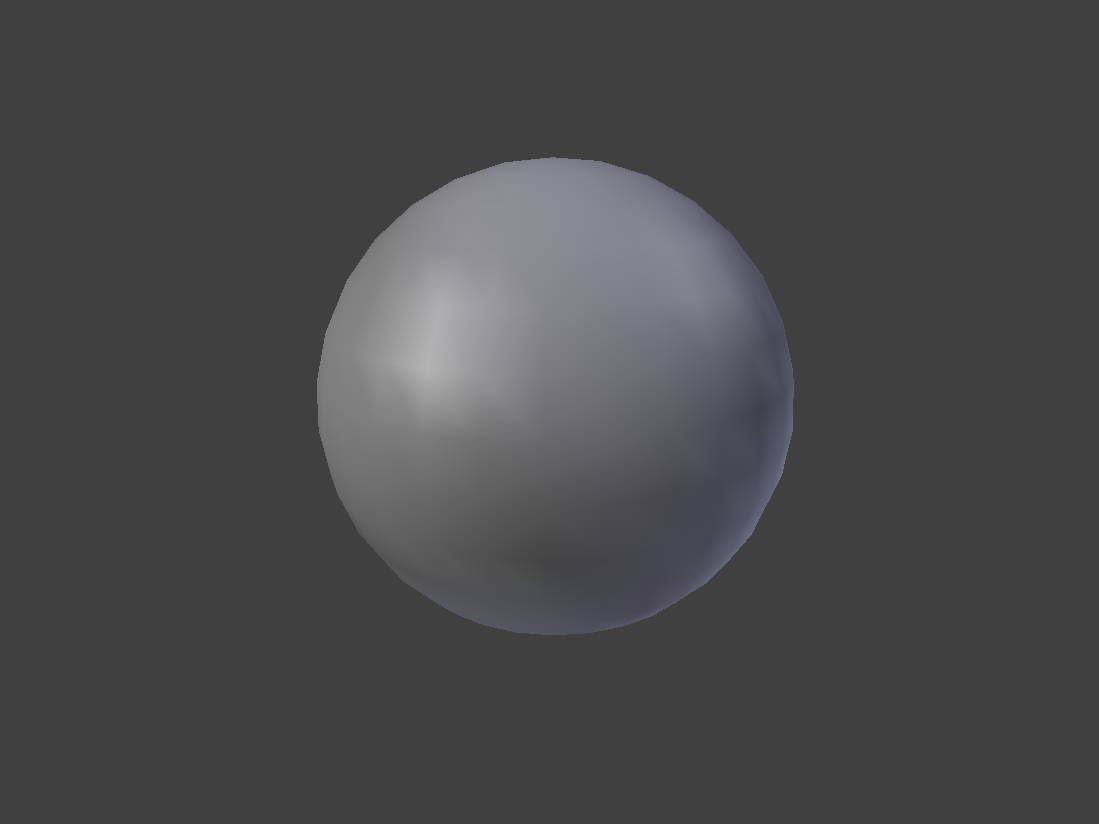
\includegraphics[width=3in]{smooth_shading.png}}

	\caption{The difference between flat and smooth shading}
	\label{fig:flat-vs-smooth-shading}
\end{figure}

In order to calculate the way a surface is lit, a normal vector describing the normal of the plane on which a point on the surface sits. One approach is to use the normal of the plane on which the triangle sits, which produces results that are not smooth as shown in figure \ref{fig:flat-vs-smooth-shading}. On the other hand, an approach called Gouraud shading \parencite{gouraud71shading}, or smooth shading, aims to simulate the lighting of a smooth surface by defining a normal for each vertex, typically an average normal for all faces sharing that vertex, and then shade each vertex of the triangle, finally interpolating the colour in between to produce a smooth fade. This effect is demonstrated in \ref{fig:colour-interpolation} by defining each vertex to have one of the primary colours and then fading in between them, creating a smooth fade.

\begin{figure}
\centering
	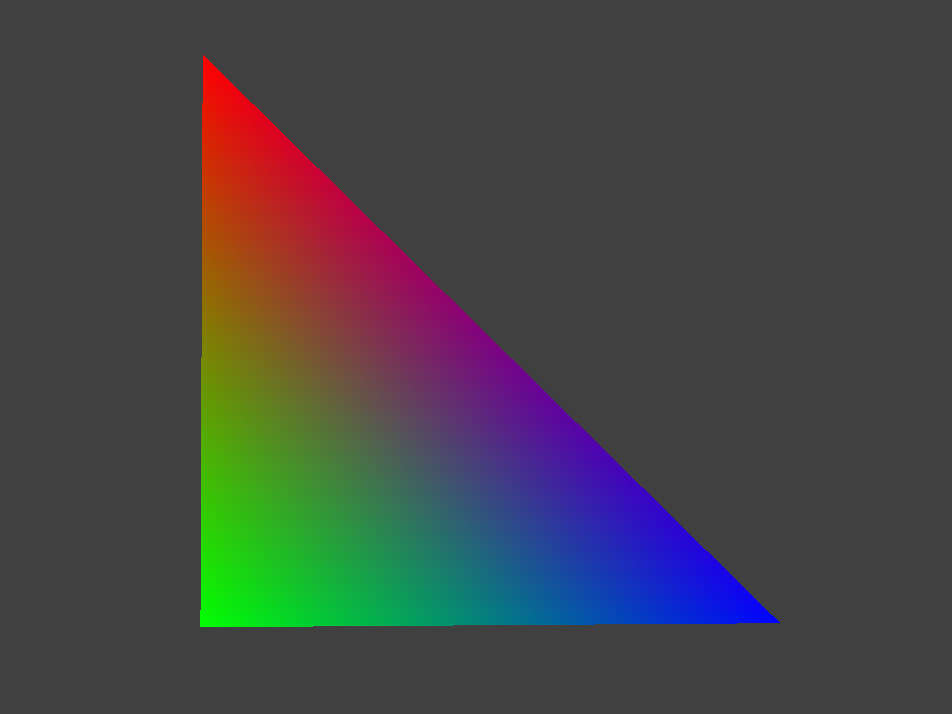
\includegraphics[width=14cm]{interpolation.png}
	\caption{Colour interpolated across a triangle}
	\label{fig:colour-interpolation}
\end{figure}


\paragraph{Ambient reflection}
Ambient reflection refers to a small amount of light which is scattered around the scene. As rasterisation-based approaches often do not consider global effects, the ambient contribution to a surface's reflection intensity, $I_{ambient}$, is typically modelled as a constant for a given scene, depending on the desired effect.

\paragraph{Diffuse reflection}

\begin{figure}
\centering
	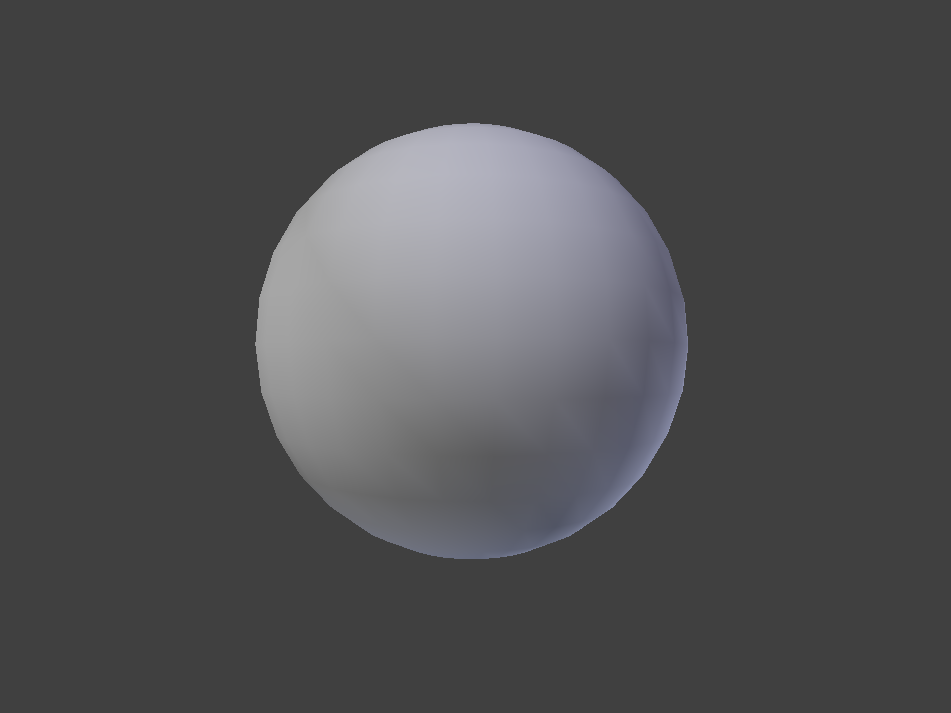
\includegraphics[width=8cm]{diffuse.png}
	\caption{An example of diffuse reflection}
	\label{fig:diffuse-reflection}
\end{figure}

Diffuse reflection refers to the scattering of light by a matte surface. Diffuse reflection is usually modelled using Lambert's cosine law, which describes the way light is scattered by a perfectly matte, or lambertian, surface.

Using Lambert's cosine law, the intensity of reflected light due to lambertian reflectance, $I_{diffuse}$, can be calculated by taking the dot product of the normalised light-direction vector $\vec{L}$ with the surface normal $\vec{N}$, as below:

\[
	I_{diffuse} = \vec{L} \cdot \vec{N}
\]

This value can then be multiplied by the colour of the surface and the intensity of the incoming light in order to determine the overall diffuse component of the surface's reflection.

\paragraph{Specular reflection}

\begin{figure}
\centering
	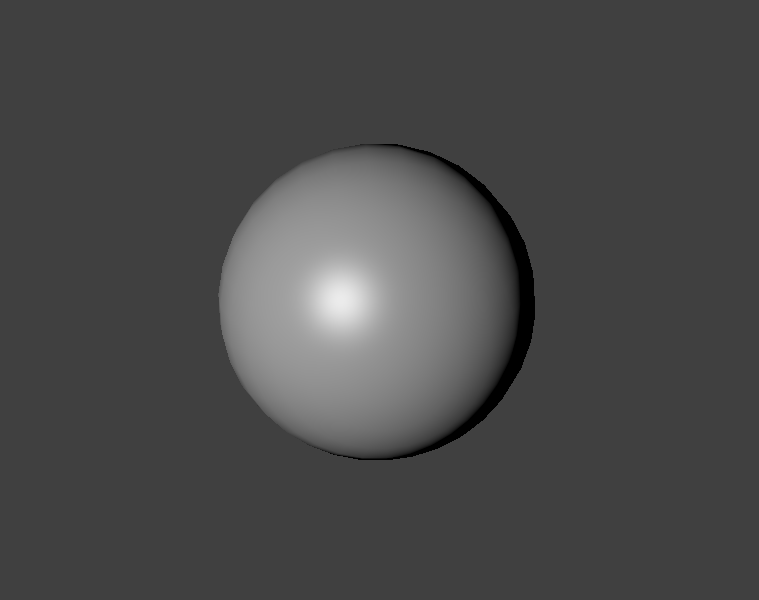
\includegraphics[width=8cm]{specular.png}
	\caption{The shiny look of this sphere is caused by specular reflection}
	\label{fig:specular-reflection}
\end{figure}

Specular reflection refers to the bright spots of light that are reflected by shiny objects. Specular highlights are visible where the surface normal lies half way between the light direction and the view direction.

Two main models are used to estimate the contribution of specular reflection to the overall reflection of a surface: the Phong shading model \parencite{phong75shading}, and a computationally lighter modification known as the Blinn-Phong shading model \parencite{blinn77blinnphong}.

These approaches improve upon Gouraud shading by interpolating the normal across the triangle, rather than just the shaded colour, increasing the computational intensity of shading, but allowing smooth specular highlights to be calculated.

\begin{figure}
\centering
	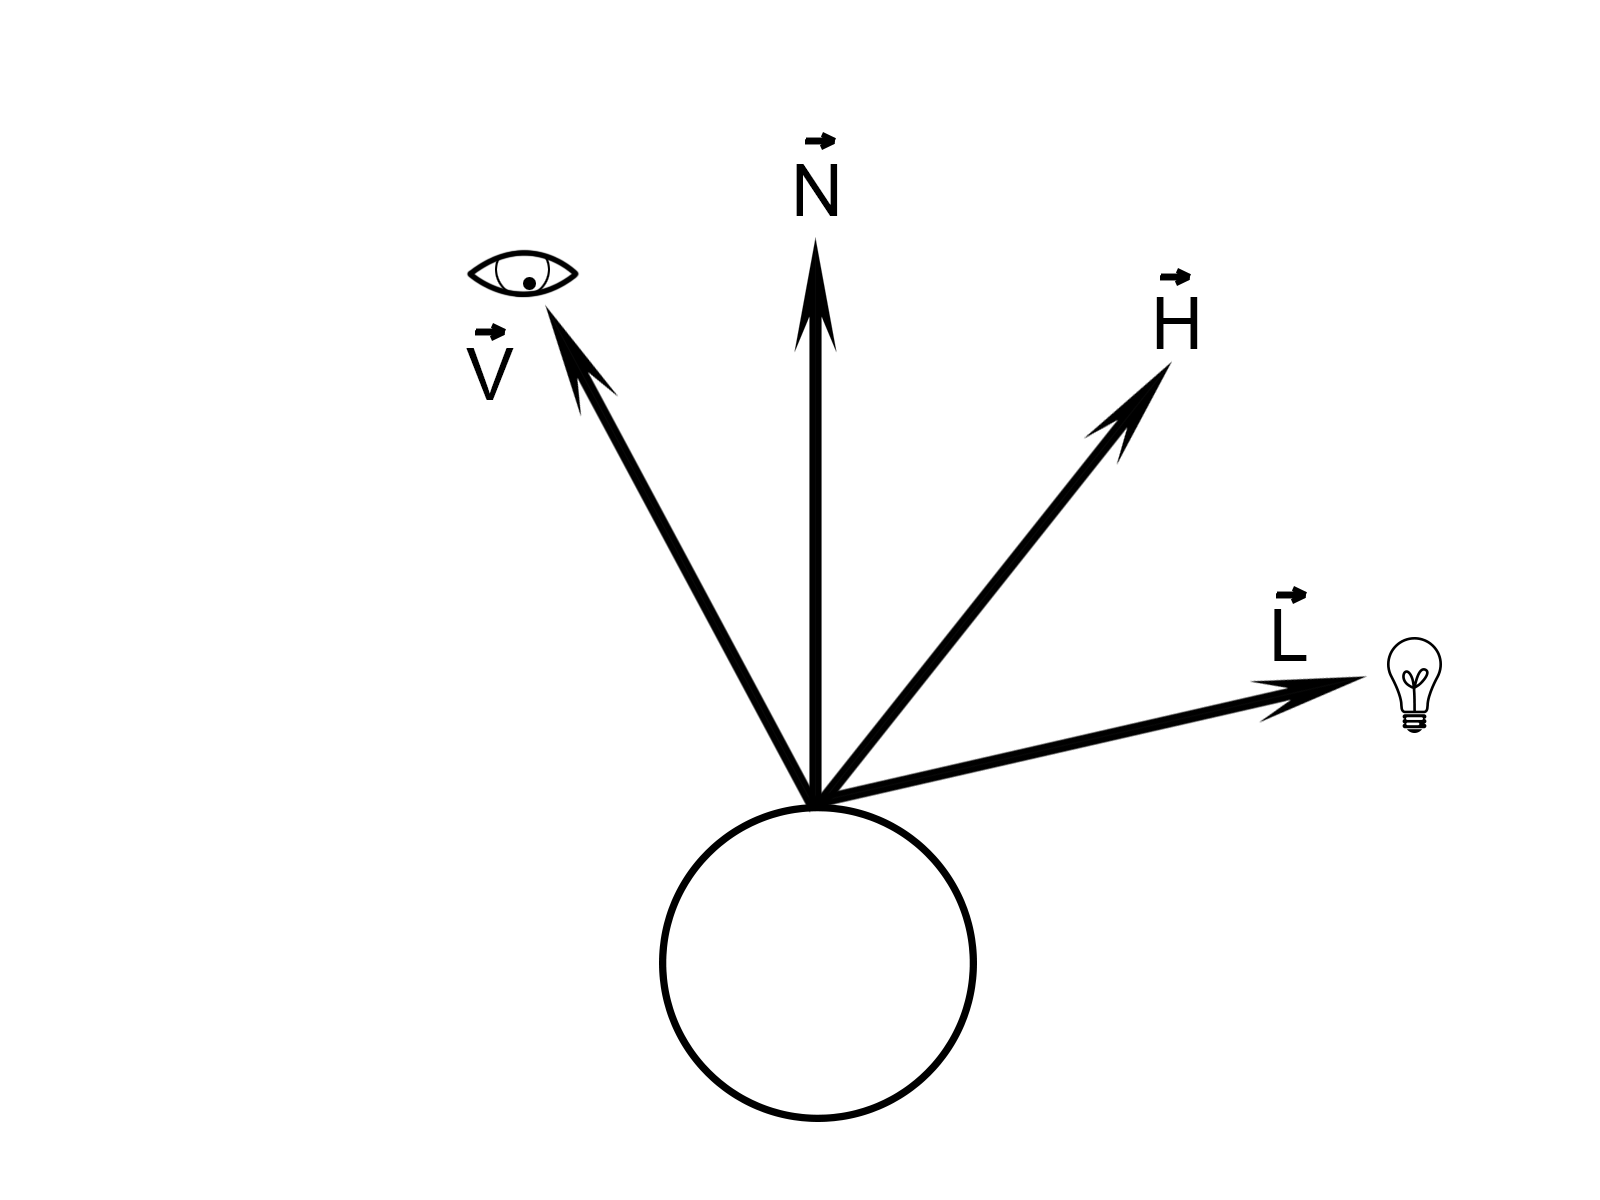
\includegraphics[width=14cm]{light_relationships.png}
	\caption{The relationship between the direction of viewing, light direction, the half-angle in between the direction of viewing and the light direction, and the normal of the surface being viewed. $\vec{L}$ is the normalised light vector which points from the surface being shaded to the light source. $\vec{N}$ is the normal of the surface being shaded. $\vec{H}$ is the direction vector half way between the angle of viewing, $\vec{V}$, and the angle of the light direction, $\vec{L}$}
	\label{fig:specular-direction-relationships}
\end{figure}

The specular component in Blinn-Phong shading is calculated by computing a half-way vector $\vec{H}$ between the view and light directions \parencite{blinn77blinnphong}:

\[
	\vec{H} = \frac{\vec{L} + \vec{V}}{|\vec{L} + \vec{V}|}
\]

Or, more simply:

\[
	\vec{H} = normalise(\vec{L} + \vec{V})
\]

This vector is shown in figure \ref{fig:specular-direction-relationships}.

The specular contribution to the overall reflection can then be calculated as:

\[
	I_{specular} = (\vec{H} \cdot \vec{N})^s
\]

Where s is the specular power, which determines the intensity of specular highlights produced by the surface. How varying the specular power affects the intensity of the specular reflections produced is shown in figure \ref{fig:specular-power}.

\begin{figure}
	\centering
	\subfloat[s = 16]{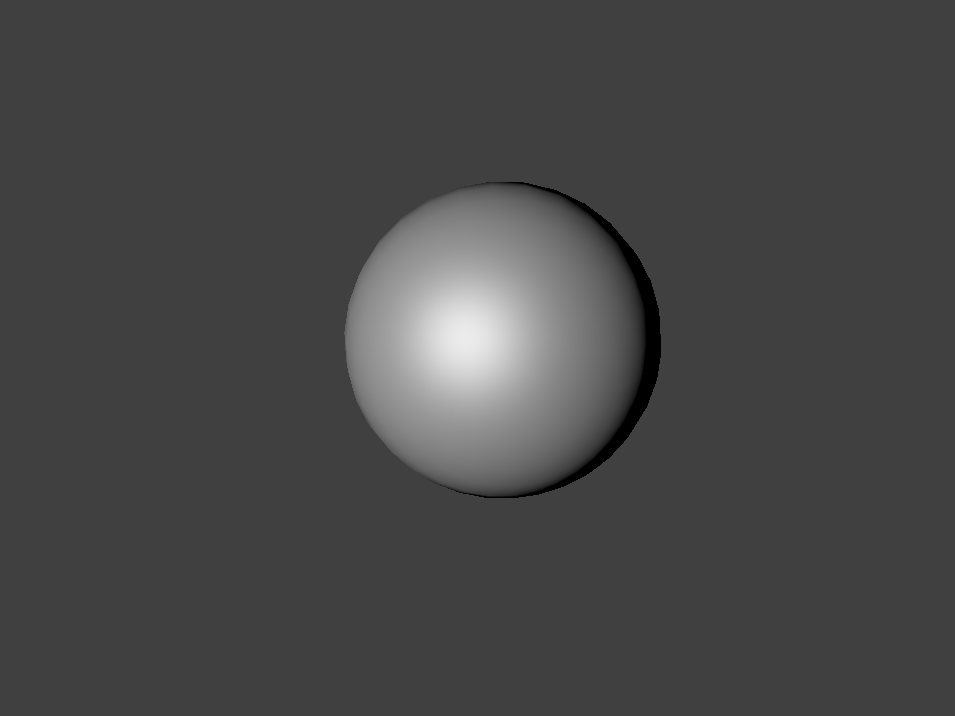
\includegraphics[width=2in]{specular_s16.png}}
	~
	\subfloat[s = 32]{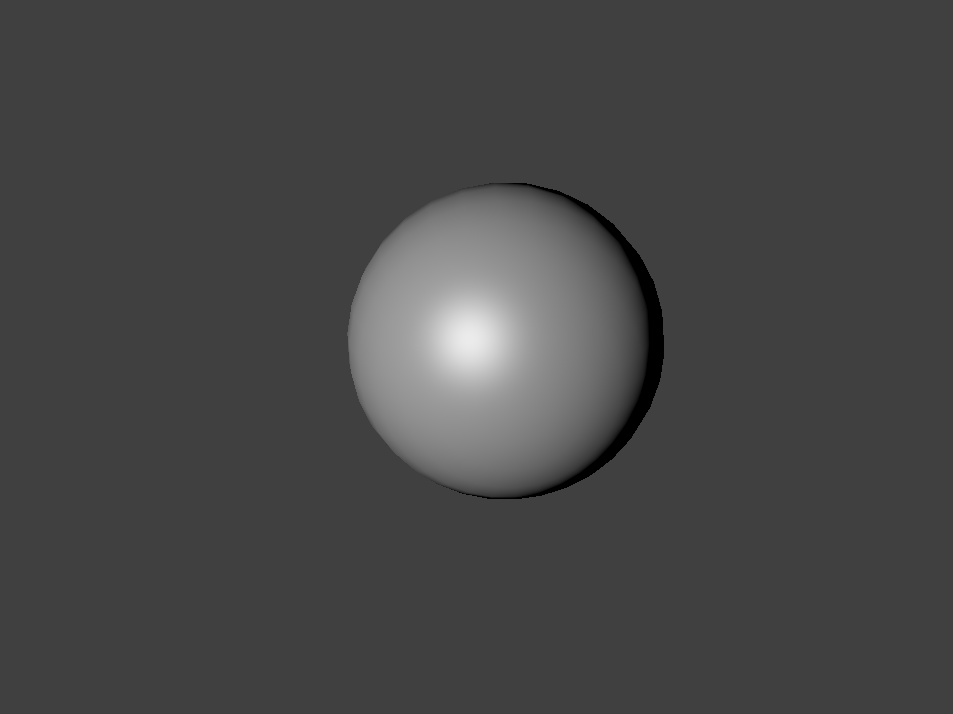
\includegraphics[width=2in]{specular_s32.png}}
	~
	\subfloat[s = 64]{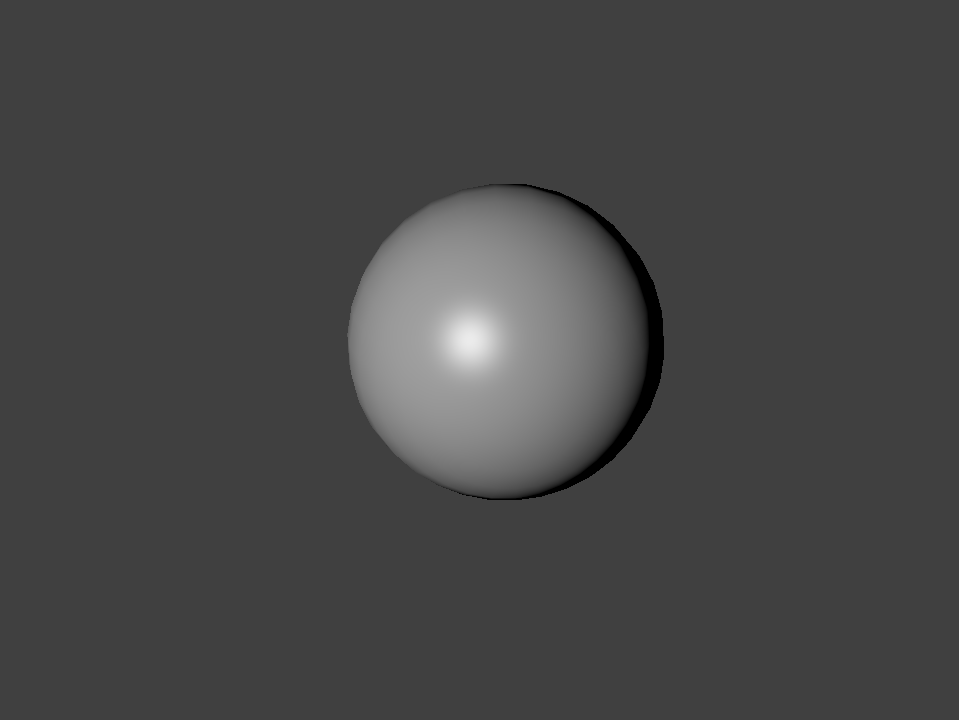
\includegraphics[width=2in]{specular_s64.png}}

	\caption{The effect of varying specular power}
	\label{fig:specular-power}
\end{figure}

\paragraph{Overall reflection}
The overall reflection of these surfaces can then be calculated additively:

\[
	I_{overall} = I_{ambient} + I_{diffuse} + I_{specular}
\]

\subsubsection{Blending}
Blending is another aspect of shading, which allows rasterised surfaces to give the appearance of partial or full transparency. By adding a fourth component to colours, an alpha component, we can define how opaque an object is, where a surface with an alpha value of 1 is fully opaque, and a surface with an alpha value of 0 is fully transparent.

By considering the alpha component of surfaces, and applying blending to additively combine the surface's colour with the background colour, the background colour is allowed to show through, as shown in figure \ref{fig:alpha-blending}.

\begin{figure}
\centering
	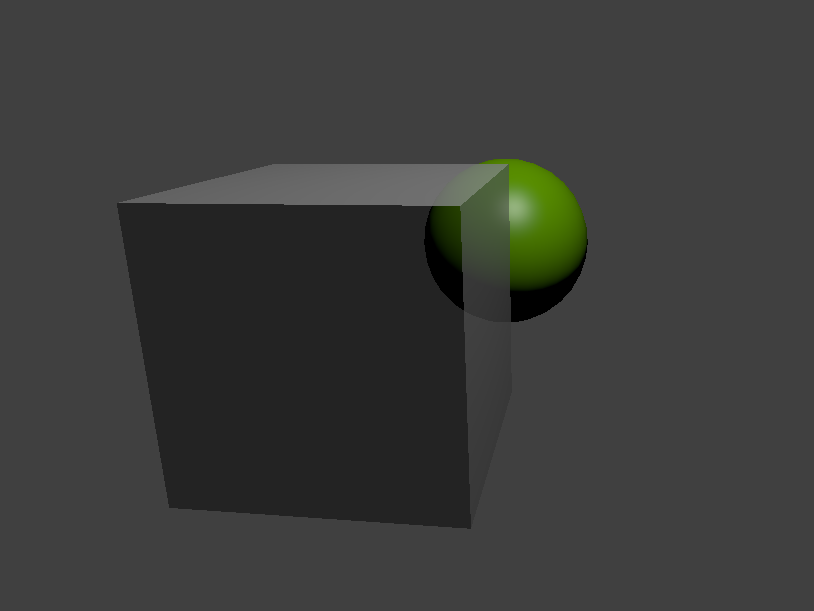
\includegraphics[width=14cm]{alpha_blending.png}
	\caption{Demonstration of alpha blending - a cube is alpha blended with the sphere in the background to give the appearance of transparency}
	\label{fig:alpha-blending}
\end{figure}

\section{Rasterisation-based volume rendering}
Researchers have used many approaches to map volume rendering operations directly to rasterisation hardware, as modern graphics hardware is extremely specialised for the purposes of rasterisation. As this sort of hardware is ubiquitous in modern computers, methods of rendering volumes in real-time using this hardware are highly sought-after. In order to understand why these approaches are not suitable for achieving our objectives, it is important to understand these approaches in order and appreciate their limitations.

\subsection{Billboards}
Billboards are texture-mapped planes which typically have no rotation component. In other words, they are always facing directly at the camera. Billboards have long since been used to render complex 3D objects in real time. By reducing complex geometry to relatively few billboards, it is possible to create a convincing enough looking representation of a 3D object. By utilising transparency and alpha blending capabilities of rasterisation hardware, it is possible to allow multiple layers of billboards to show through.

A common example as used in games is for tree rendering. A technique demonstrated by \citeauthor{garcia05tree} utilises a set of billboards, referred to in the paper as a cloud of billboards, in order to vastly simplify complicated tree models defined by hundreds of thousands of polygons into a few fixed billboards, each of which can approximate many leaves. This technique is demonstrated in figure \ref{fig:billboard-cloud-trees}.

\begin{figure}
\centering
	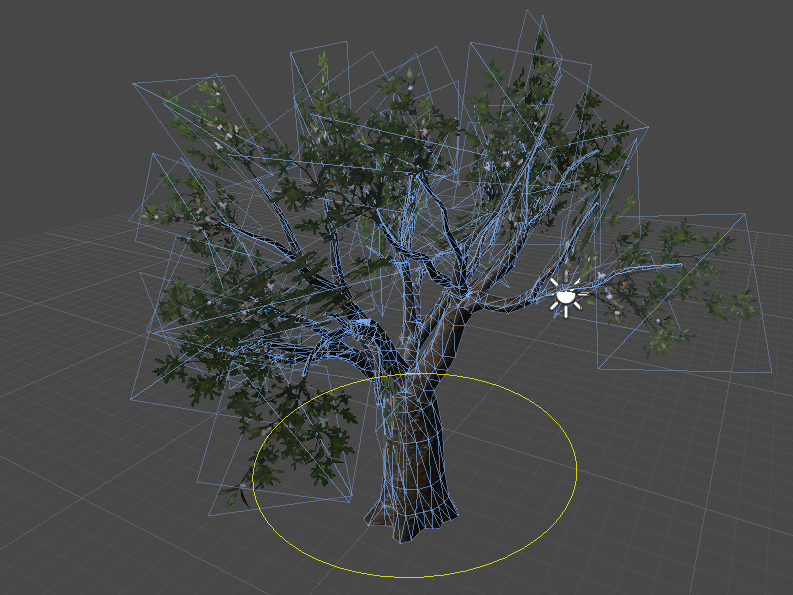
\includegraphics[width=14cm]{tree_billboards.png}
	\caption{Billboard cloud tree rendering}
	\label{fig:billboard-cloud-trees}
\end{figure}

Similar techniques have also been successfully developed for volume rendering. \cite{harris02real} combined the simulation of multiple forward scattering within a cloud volume with billboards used to accelerate rendering. By utilising impostors, billboards subtly intended to replace 3D objects, this approach accelerates rendering by rendering to the billboards and reusing the results between frames. This method allows for realistic real-time rendering of clouds.

The limitation of this approach is that it does not simulate global effects, and as such, the rest of the scene does not have an effect on the rendering of an individual cloud volume. In fact, the cloud rendering approach utilised in this paper is very specific in the effects which it simulates, simulating very homogeneous looking clouds that are not affected very much by the scene or surrounding clouds. Although this may be a suitable compromise for some games, it falls short of our objectives to simulate true volumetric effects in real-time. Nonetheless, the impostor technique may be suitable in some cases in order to exploit frame-to-frame coherence.

\subsection{Texture-based approaches}
\cite{engel02interactivehigh-quality} proposes an approach that utilises a 3D texture as proxy geometry, exploiting hardware alpha blending as a means to composite overlapping samples in order to create a 3D image of a volume.

The advantage of this approach is that it maps onto existing rasterisation hardware very well, allowing real-time volume rendering on relatively cheap, ubiquitous graphics hardware. The major limitation of this method, however, is that it only considers overlapping parts of the volume. If one wishes to calculate lighting effects which involve light being reflected or refracted in different directions as we do, this approach is not suitable. In addition, \citeauthor{engel02interactivehigh-quality} found the precision of rasterisation hardware limited when it came to texture representations, which resulted in artifacts in the rendered image.

\begin{algorithm}
\caption{Per-pixel rendering}
\label{alg:render}
\begin{algorithmic}[1]
\Procedure{render\_pixel}{$x, y, tree, projection$}
	\State $out\_colour \gets (0, 0, 0, 0)$
	\State $ray \gets calculate\_ray(x,~y,~projection)$
	\State $intersection \gets \Call{raycast}{tree, ray}$
	\If{$intersection.hit$}
		\State $out\_colour \gets \Call{shade}{tree,~ ray,~ intersection}$
	\EndIf
	\State $\textbf{return} out_colour$
\EndProcedure
\\
\Procedure{shade}{$tree,~ ray,~ intersection$}
	\State $out\_colour \gets (0, 0, 0, 0)$
	\For{$each~light$} \Comment{Shade for each light}
		\State $light\_dir \gets light\_pos - intersection.position$ \Comment{Check shadow}
		\State $shadow\_ray \gets (intersection.position, light_dir)$
		\State $shadow\_intersection \gets \Call{raycast}{tree, shadow\_ray}$
		\If{$shadow\_intersection.hit$}
			\State $\textbf{continue}$
		\EndIf
		\State $out\_colour ~+=~ \Call{diffuse\_reflection}{intersection,~light}$
		\State $out\_colour ~+=~ \Call{specular\_reflection}{intersection,~light}$
	\EndFor
	\\
	\State $reflection\_ray \gets \Call{reflect}{ray,~intersection}$ \Comment{Reflection}
	\State $reflection\_intersection \gets \Call{raycast}{tree, reflection\_ray}$
	\If{$reflection\_intersection.hit$}
		\State $out\_colour ~+=~ \Call{shade}{tree,~ reflection\_ray,~ reflection\_intersection}$
	\EndIf
	\\
	\State $refraction\_ray \gets \Call{refract}{ray,~intersection}$ \Comment{Refraction}
	\State $refraction\_intersection \gets \Call{raycast\_empty}{tree, refraction\_ray}$
	\If{$refraction\_intersection.hit$}
		\State $out\_colour ~+=~ \Call{shade}{tree,~ refraction\_ray,~ refraction\_intersection}$
	\EndIf
\EndProcedure
\end{algorithmic}
\end{algorithm}

\section{Ray tracing}
A more generic approach called ray tracing, similar to the approach in \cite{engel02interactivehigh-quality}, aims to simulate the path of light in reverse. Ray tracing starts by firing rays outwards into the scene from the camera \parencite{appel68raytracing}, traditionally firing one ray per pixel and finding the first intersection of the scene with the ray.

\begin{figure}
\centering
	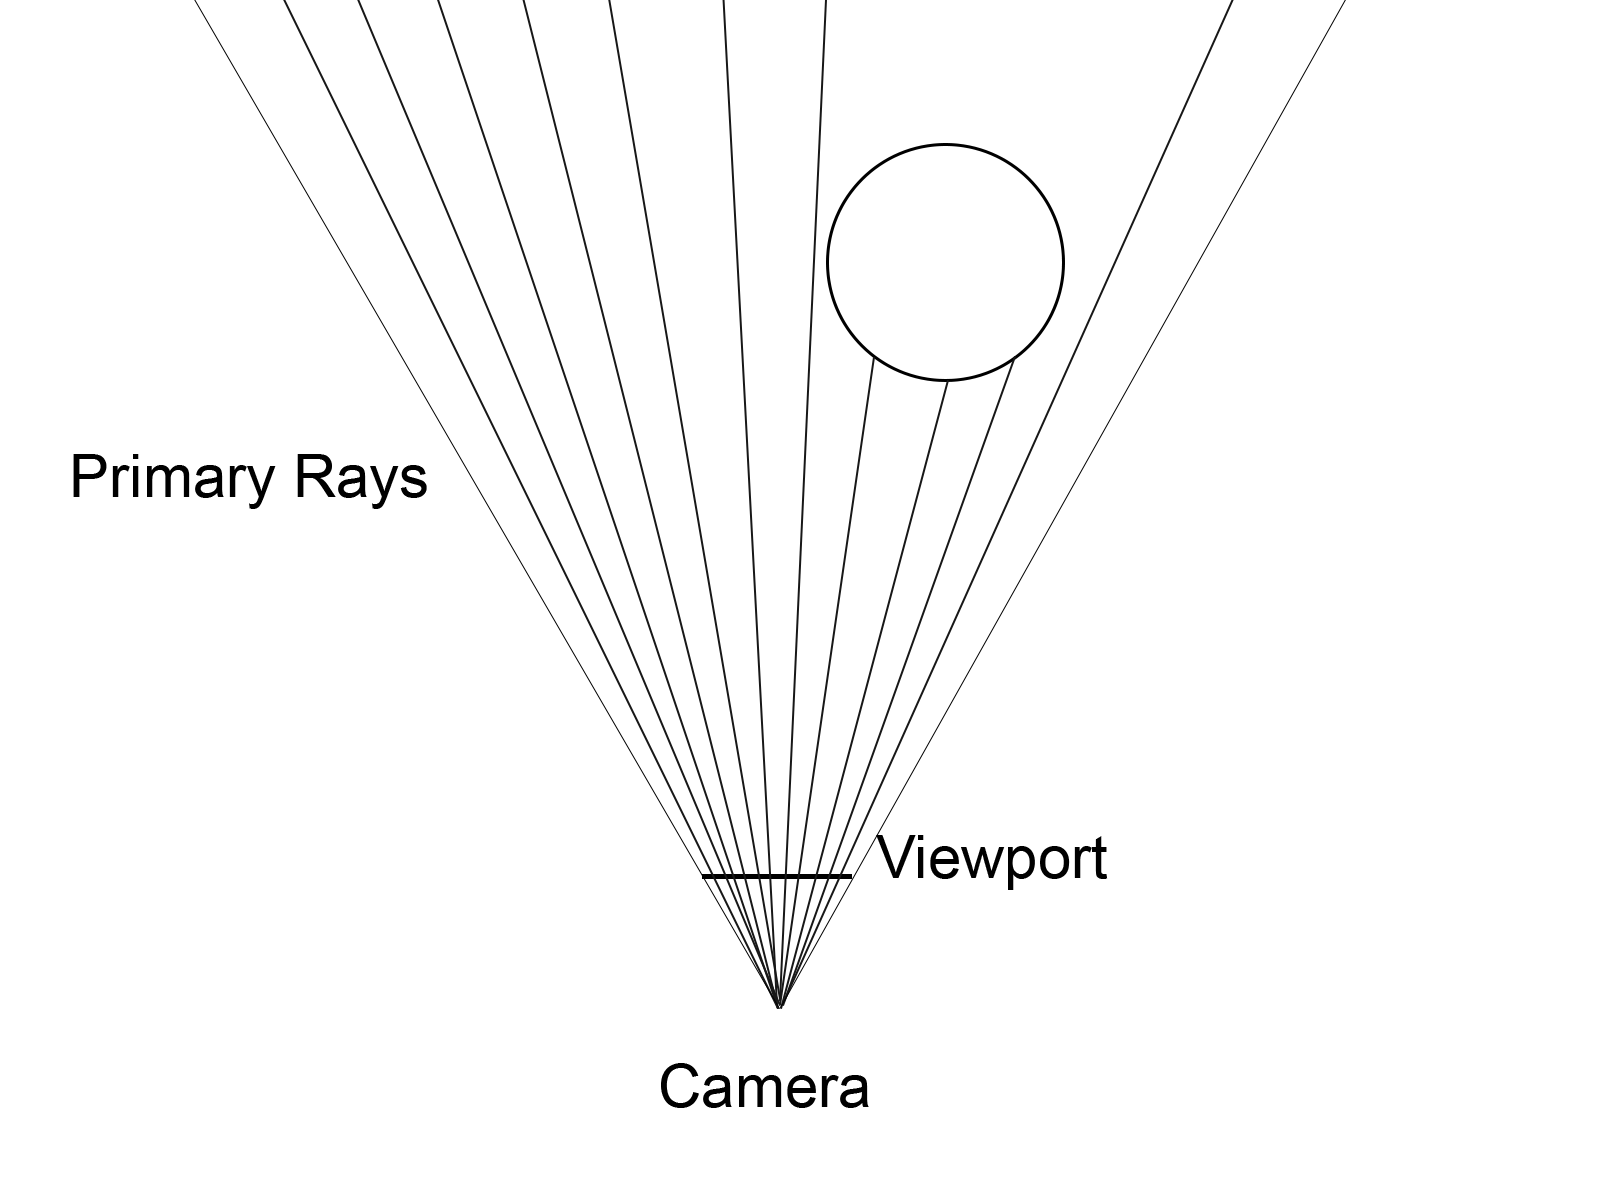
\includegraphics[width=14cm]{primaryray.png}
	\caption{In ray tracing, primary rays are cast through each pixel on the viewport}
	\label{fig:primaryray}
\end{figure}

Once an intersection is found, additional rays can be spawned in order to take account of the effects of reflection and refraction. Unlike \citeauthor{engel02interactivehigh-quality}'s approach, this allows the ray of light to follow a path that isn't just straight, allowing rendering to account for the contribution to lighting of other parts of the scene that aren't directly overlapping a particular pixel.

\begin{figure}
\centering
	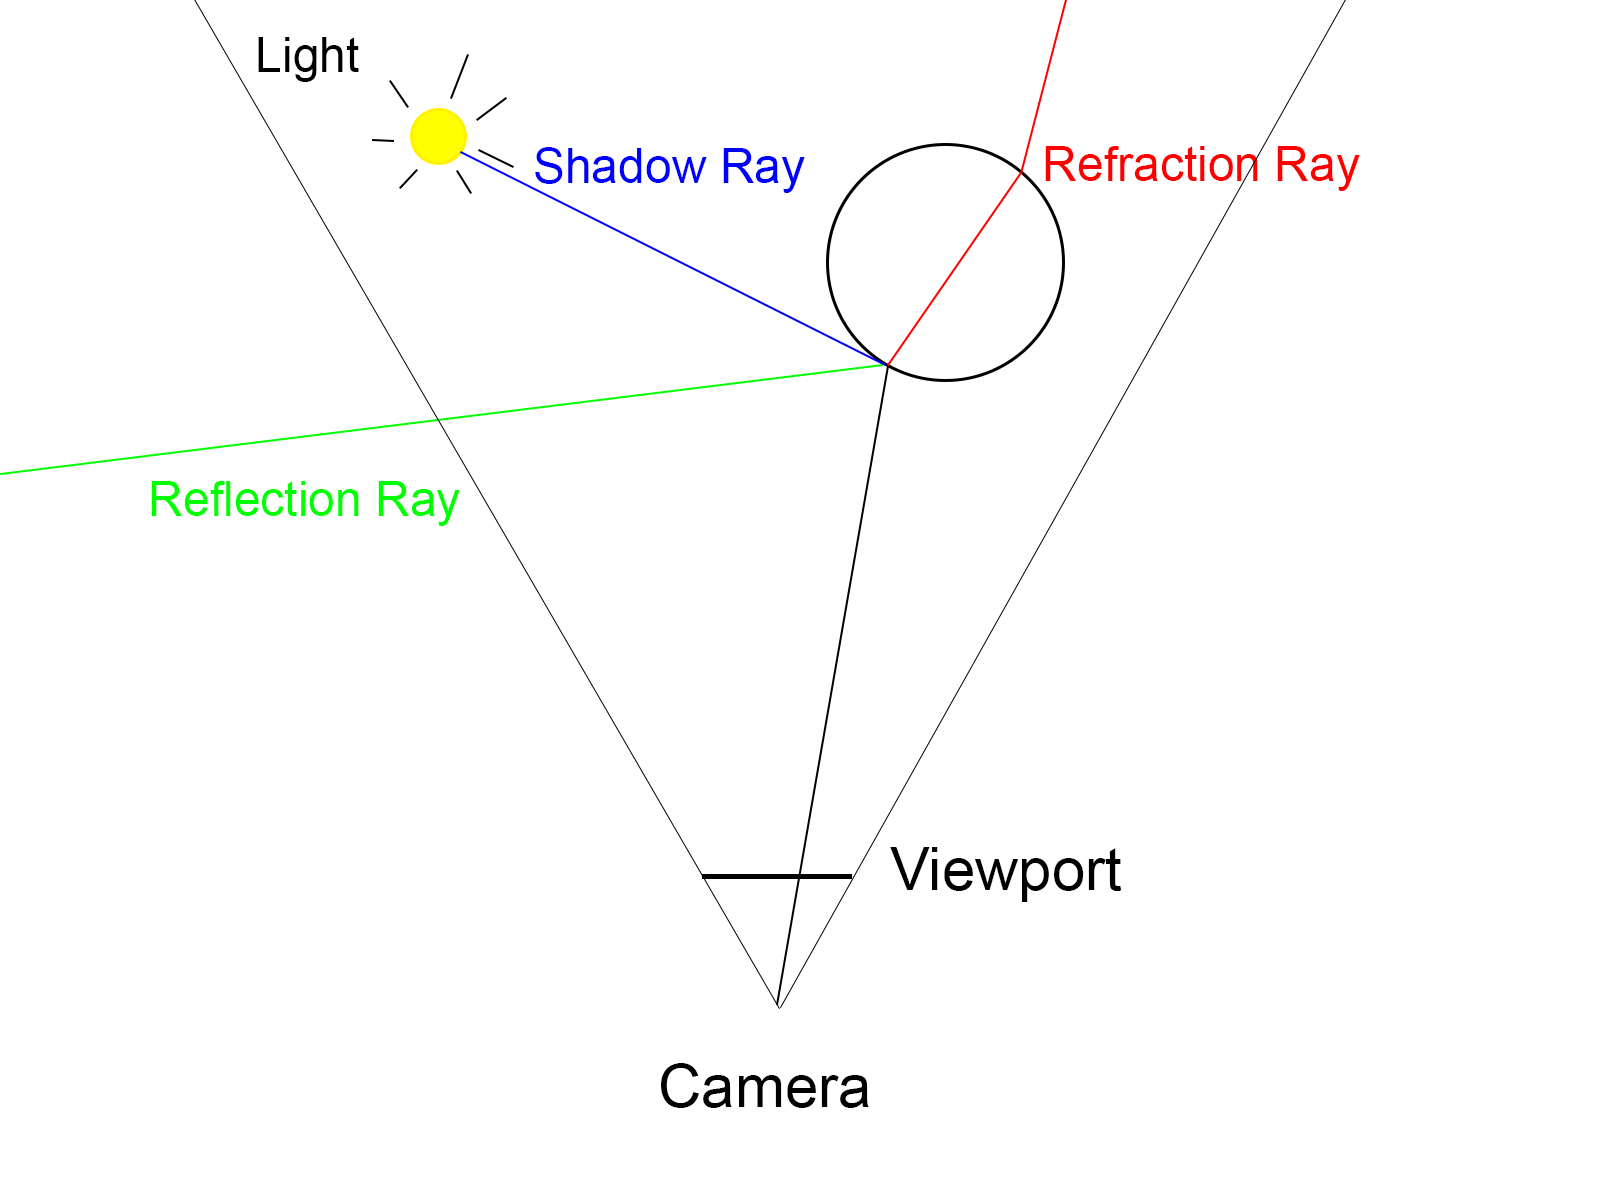
\includegraphics[width=14cm]{secondaryrays.png}
	\caption{Additional rays can then be spawned for each intersection to calculate shadow coverage, reflection, and refraction}
	\label{fig:secondaryrays}
\end{figure}

In addition to allowing light reflected from the rest of the scene to be taken into account, rays can also peer directly into volumes in order to determine the effects of lighting within them. This allows us to consider volumes that are not just homogeneous in nature, as the ray can be affected within the volume by the internal structure of the volume.

\subsection{Direct volume rendering}
Ray tracing allows the direct rendering of a volume, without having to first sample the underlying volume into another format. Any volume (or structure) for which an intersection test can be defined can be rendered by means of ray tracing. 

\cite{roth82roughimprove} presented an algorithm for directly rendering constructive solid geometry (CSG), a method for representing 3D shapes which involves combining various geometric shapes using boolean operations. This work described the calculation of eye rays for orthographic as well as perspective projections, as well as a hierarchical data structure for storing and rendering CSG directly. This work also described a number of primitives as well as the relevant necessary intersection tests. Additionally, \citeauthor{roth82roughimprove} demonstrated the application of this algorithm for producing realistically shaded solids for use in computer aided design, and also used shadow rays in order to produce ray traced shadows, and even described a method for anti-aliasing of the resulting image.

The direct rendering of volumes simplifies computation, removing the need for us to rely on intermediate representations of volumes, and allowing us to consider the volume itself as all information may be relevant to the rendering of the current pixel.

Although this allows broad coverage of geometric shapes, it is difficult to represent highly heterogeneous volumes with CSG, as it would require a very large number of separate geometric shapes to model changes in heterogeneous attributes. In addition, it would be impossible to render smoothly changing heterogeneous attributes without a very large number of geometric shapes, at which point it would be more efficient to use a grid-based sampling approach. For this reasons, it is unsuitable for our objectives.

\subsection{Space subdivision}
The next important advancement in ray casting technology was presented by~\cite{glassner84space}. By using an octree, a hierarchical volume representation, to partition space, and storing a list of objects in each node of the tree, he greatly reduced the number of comparisons required for each ray. This allowed the rendering of hundreds, or even thousands of objects in a scene without greatly increasing the computation time for each object. Despite this, an object format which is capable of storing heterogeneous volumes is still required.

On the other hand, \cite{wilhelms00octreesfor} presented a space-efficient octree representation that is designed for representing voxel data directly. By not storing empty space within the tree, a technique referred to as sparse voxel octrees (SVOs), a considerable amount of space is saved, reducing the memory footprint of the stored voxel data. Additionally, as the voxel data is stored directly using this kind of approach, it is possible to represent heterogeneous volumes with this structure.

\cite{amanatides87afast} presented a significant optimisation to the traditional ray tracing algorithm, by presenting a method of mathematically determining the next voxel in a traversal and automatically stepping directly to its boundary. Using this new algorithm, traversing from one voxel to its neighbour requires only two floating point comparisons and one floating point addition. This greatly reduces computation time for ray casts, and is the basis for a large amount of derivative work on efficient ray casting.

\cite{arvo88octreewalking} extends this technique to the octree, presenting an efficient linear-time voxel walking algorithm for octrees with a best case complexity of O(log N). \citeauthor{arvo88octreewalking}'s approach is a top-down approach which ensures that nodes are only considered once per ray and visits the voxels in the correct order, resulting in the O(log N) best case complexity. \citeauthor{arvo88octreewalking}'s algorithm involves checking the intersection of the ray with the root node of the octree, and recursively shortening the spans of the ray that are considered for intersection.

\subsection{GPU implementation}
Due to the fact that ray tracing utilises one primary ray per pixel, a fact that both limits it and works to its advantage in its basic implementation, the process is highly parallelisable. Additionally over the last decade, a breakthrough occurred in graphics hardware, which saw GPUs becoming massively parallel general-purpose stream processors, as opposed to the original fixed-function format. \cite{purcell02gpuraytracing} investigates this trend and explains how ray tracing can be mapped to graphics hardware. \citeauthor{purcell02gpuraytracing} demonstrate how to reformulate ray tracing as a streaming computation, making it appropriate for GPU implementation. The process is as follows:

% Hide number from itemize list item
\let\oldlabelitemi\labelitemi
\renewcommand{\labelitemi}{}

\begin{itemize}
	\item For each pixel of the screen:

	\begin{enumerate}
		\item Generate eye rays
		\item Traverse acceleration structure

			\begin{enumerate}
				\item Do intersection tests
			\end{enumerate}

		\item Shade hit

			\begin{enumerate}
				\item Generate shading rays (repeating 2-3 as necessary)
			\end{enumerate}

	\end{enumerate}
\end{itemize}

\citeauthor{purcell02gpuraytracing} were the first to demonstrate that efficient real-time ray tracing in the GPU is possible without any changes in architecture.

% Restore old itemize list item style
\let\labelitemi\oldlabelitemi

\subsection{Efficient GPU traversal}
\cite{aila2009hpg} discusses the mapping of elementary ray tracing operations such as traversal and intersection onto GPUs. This work focuses on understanding the efficiency of GPU ray traversal rather than directly presenting an efficient ray traversal implementation, highlighting the fact that very little is understood about the performance of fast ray traversal algorithms. By comparing the performance of these algorithms against a theoretical upper bound, \citeauthor{aila2009hpg} demonstrate that previous methods are off by a factor of 1.5x - 2.5x theoretical optimal performance, and highlight previously unidentified inefficiencies in hardware work distribution.

Their work demonstrates that reliance on persistent threads rather than hardware work distribution mechanisms can improve the performance of the fastest GPU trace() kernels significantly.

\subsection{Efficient octree storage}
\cite{wilhelms00octreesfor} present a space-efficient octree representation that does not allocate memory for empty space - what has become known as a sparse voxel octree (SVO). \citeauthor{wilhelms00octreesfor}'s structure utilises a pointer-less "linear octree" structure which avoids storing pointers between every node.

\cite{laine10efficientsvos} expand on these ideas by storing pointers between blocks of octrees and otherwise determining a particular child's address using an index and a parent's 8-bit child mask. As the child's pointer can be obtained from a lookup table using this index and child mask, it is unnecessary to store a pointer for every voxel, making the structure far more efficient.

As \citeauthor{laine10efficientsvos} demonstrate, the SVO structure can be efficiently ray traced with an implicit level of depth (LOD) mechanism, as traversal can be terminated as soon as a found voxel is smaller than the current pixel on the screen. At high resolutions, however, even with the efficient SVO storage structure presented by \citeauthor{laine10efficientsvos}, mid-sized scenes still take up an excessive amount of storage, with \citeauthor{laine10efficientsvos}'s test scenes utilising up to 4GBs of memory, the upper bounds of memory on today's GPUs.

However, while extremely efficient to ray cast, and fairly compact when compared to other structures, \citeauthor{laine10efficientsvos}'s structure is still fairly heavy on memory usage. In their paper, \citeauthor{laine10efficientsvos} address this by only encoding surfaces, an approach that is obviously not possible if volumetric effects are desired.

To combat memory usage, they additionally implement a concept called contours, in which surface voxels are restrained to a non-cubic shape using a pair of parallel planes, and once this shape provides a good enough approximation of the surface, the tree does not need to be generated any further. \citeauthor{laine10efficientsvos}'s implementation for this is very efficient, and automatically takes into account multiple levels of contours in order to produce a shape extremely close to the source data. A similar process could also be used to prevent unnecessary depth in homogeneous regions, where the current approximation of the volume is sufficiently good.

Additionally, more recent work by \citeauthor{kampe2013dags} has greatly reduced the memory usage of SVOs by allowing identical regions of the tree to share pointers, allowing the reuse of data between regions. This new structure is referred to as a direct analytic graph, or sparse voxel DAG. \citeauthor{kampe2013dags} have found that, using this technique, the memory usage of even highly irregular scenes can be reduced by 1 to 3 orders of magnitude. Despite this being most effective for more homogeneous scenes, the gains shown for highly irregular scenes are also very promising.

\subsection{Animation}
Due to the nature of deformation, animation has previously not been possible with voxel structures because it would leave gaps between voxels. Additionally, deforming a hierarchical structure means that there is no longer a guarantee that all child nodes lie inside their parent nodes. \cite{bautembach2011animated} presented an approach to the animation of voxel octrees by expanding the parent voxels so that they still encompass all child voxels. \citeauthor{bautembach2011animated}'s approach demonstrates an efficient and effective approach capable of character animation with sparse voxel octrees, something which had previously been considered infeasible.

\subsection{Caching}
\cite{ruff13dynamiccaching} presented a caching-like strategy which is capable of storing data generated in previous frames which can then be used to accelerate rendering in later frames. \citeauthor{ruff13dynamiccaching} claim that their approach can be integrated to any existing ray tracing solution, and will allow data to be reused between frames. A significant limitation of this approach, however, is that it is tailored to static scenes. \citeauthor{ruff13dynamiccaching} point out that any movement of the scene objects would generate inconsistencies in cached data, although they do provide some potential solutions to this problem.

\subsection{Limitations of ray tracing}

\begin{figure}
\centering
	\centering
	\subfloat[hard shadows]{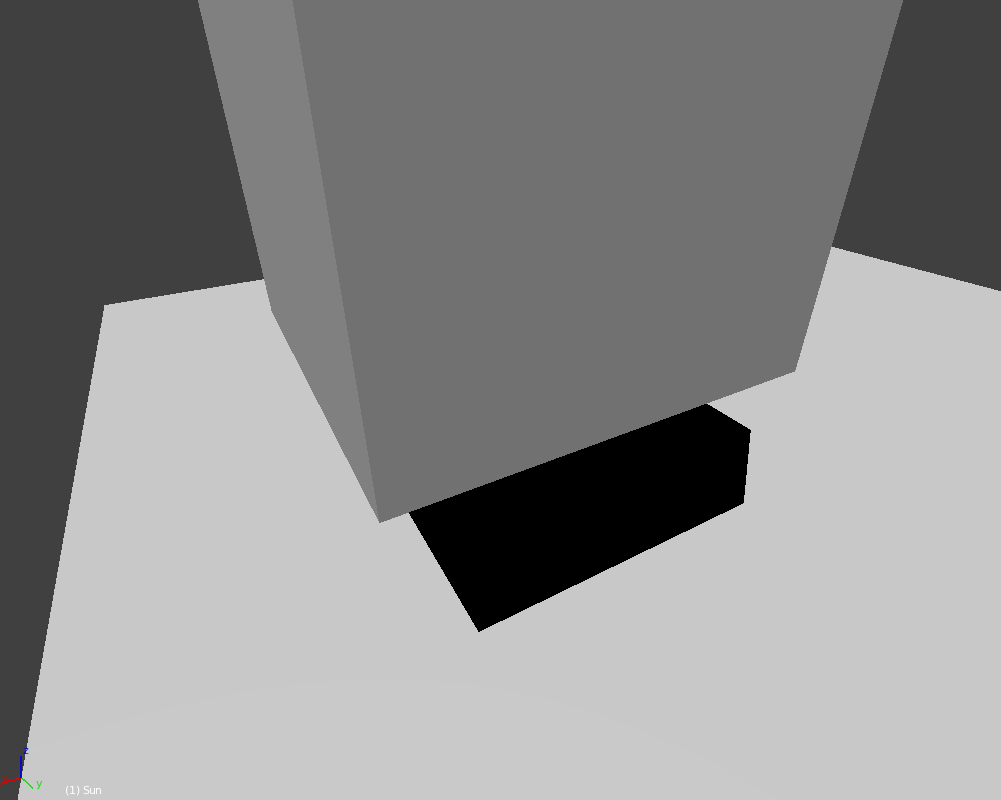
\includegraphics[width=3in]{hard_shadows.png}}
	~
	\subfloat[soft shadows]{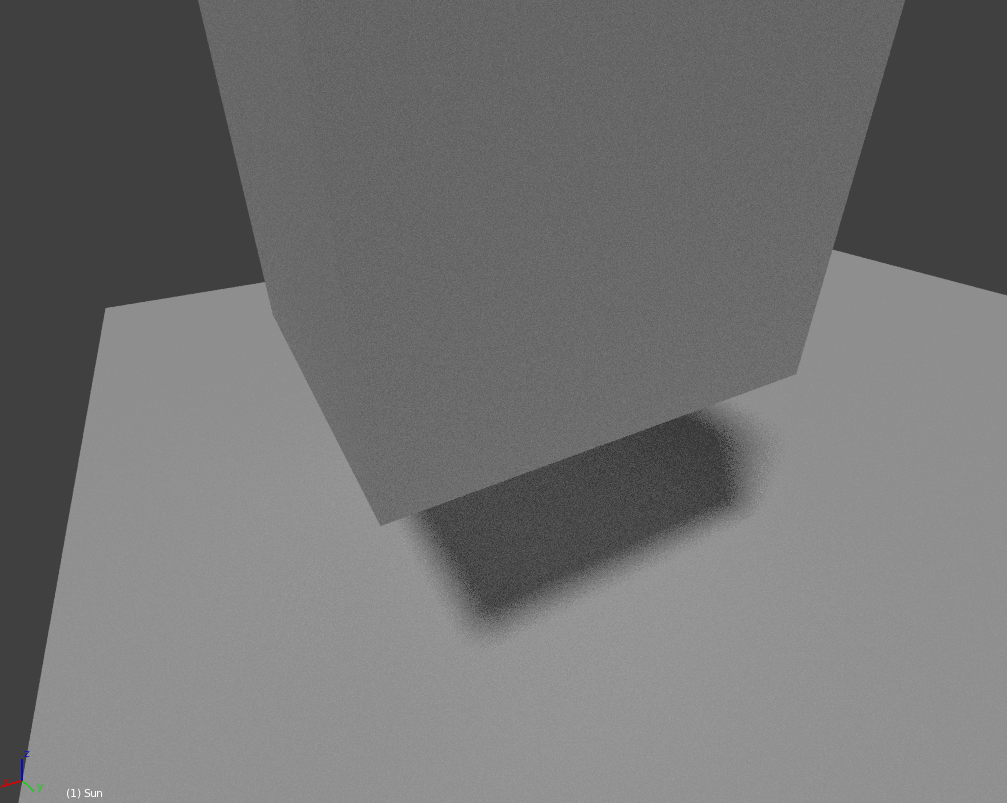
\includegraphics[width=3in]{soft_shadows.png}}

	\caption{The hard edges of shadows generated by ray tracing, next to the soft shadows created by path tracing}
	\label{fig:shadow-hard-edge}
\end{figure}

Despite the numerous advantages of ray tracing, it has one major disadvantage: ray tracing can not simulate fuzzy phenomena, such as soft shadows. Figure \ref{fig:shadow-hard-edge} demonstrates shadows as simulated by ray tracing. Shadows produced by ray tracing are defined by explicit boundaries, where in real life, the edges of shadows are not well defined. In order to understand why ray tracing has this limitation, it is important to understand exactly what it is trying to approximate.

\begin{figure}
\centering
	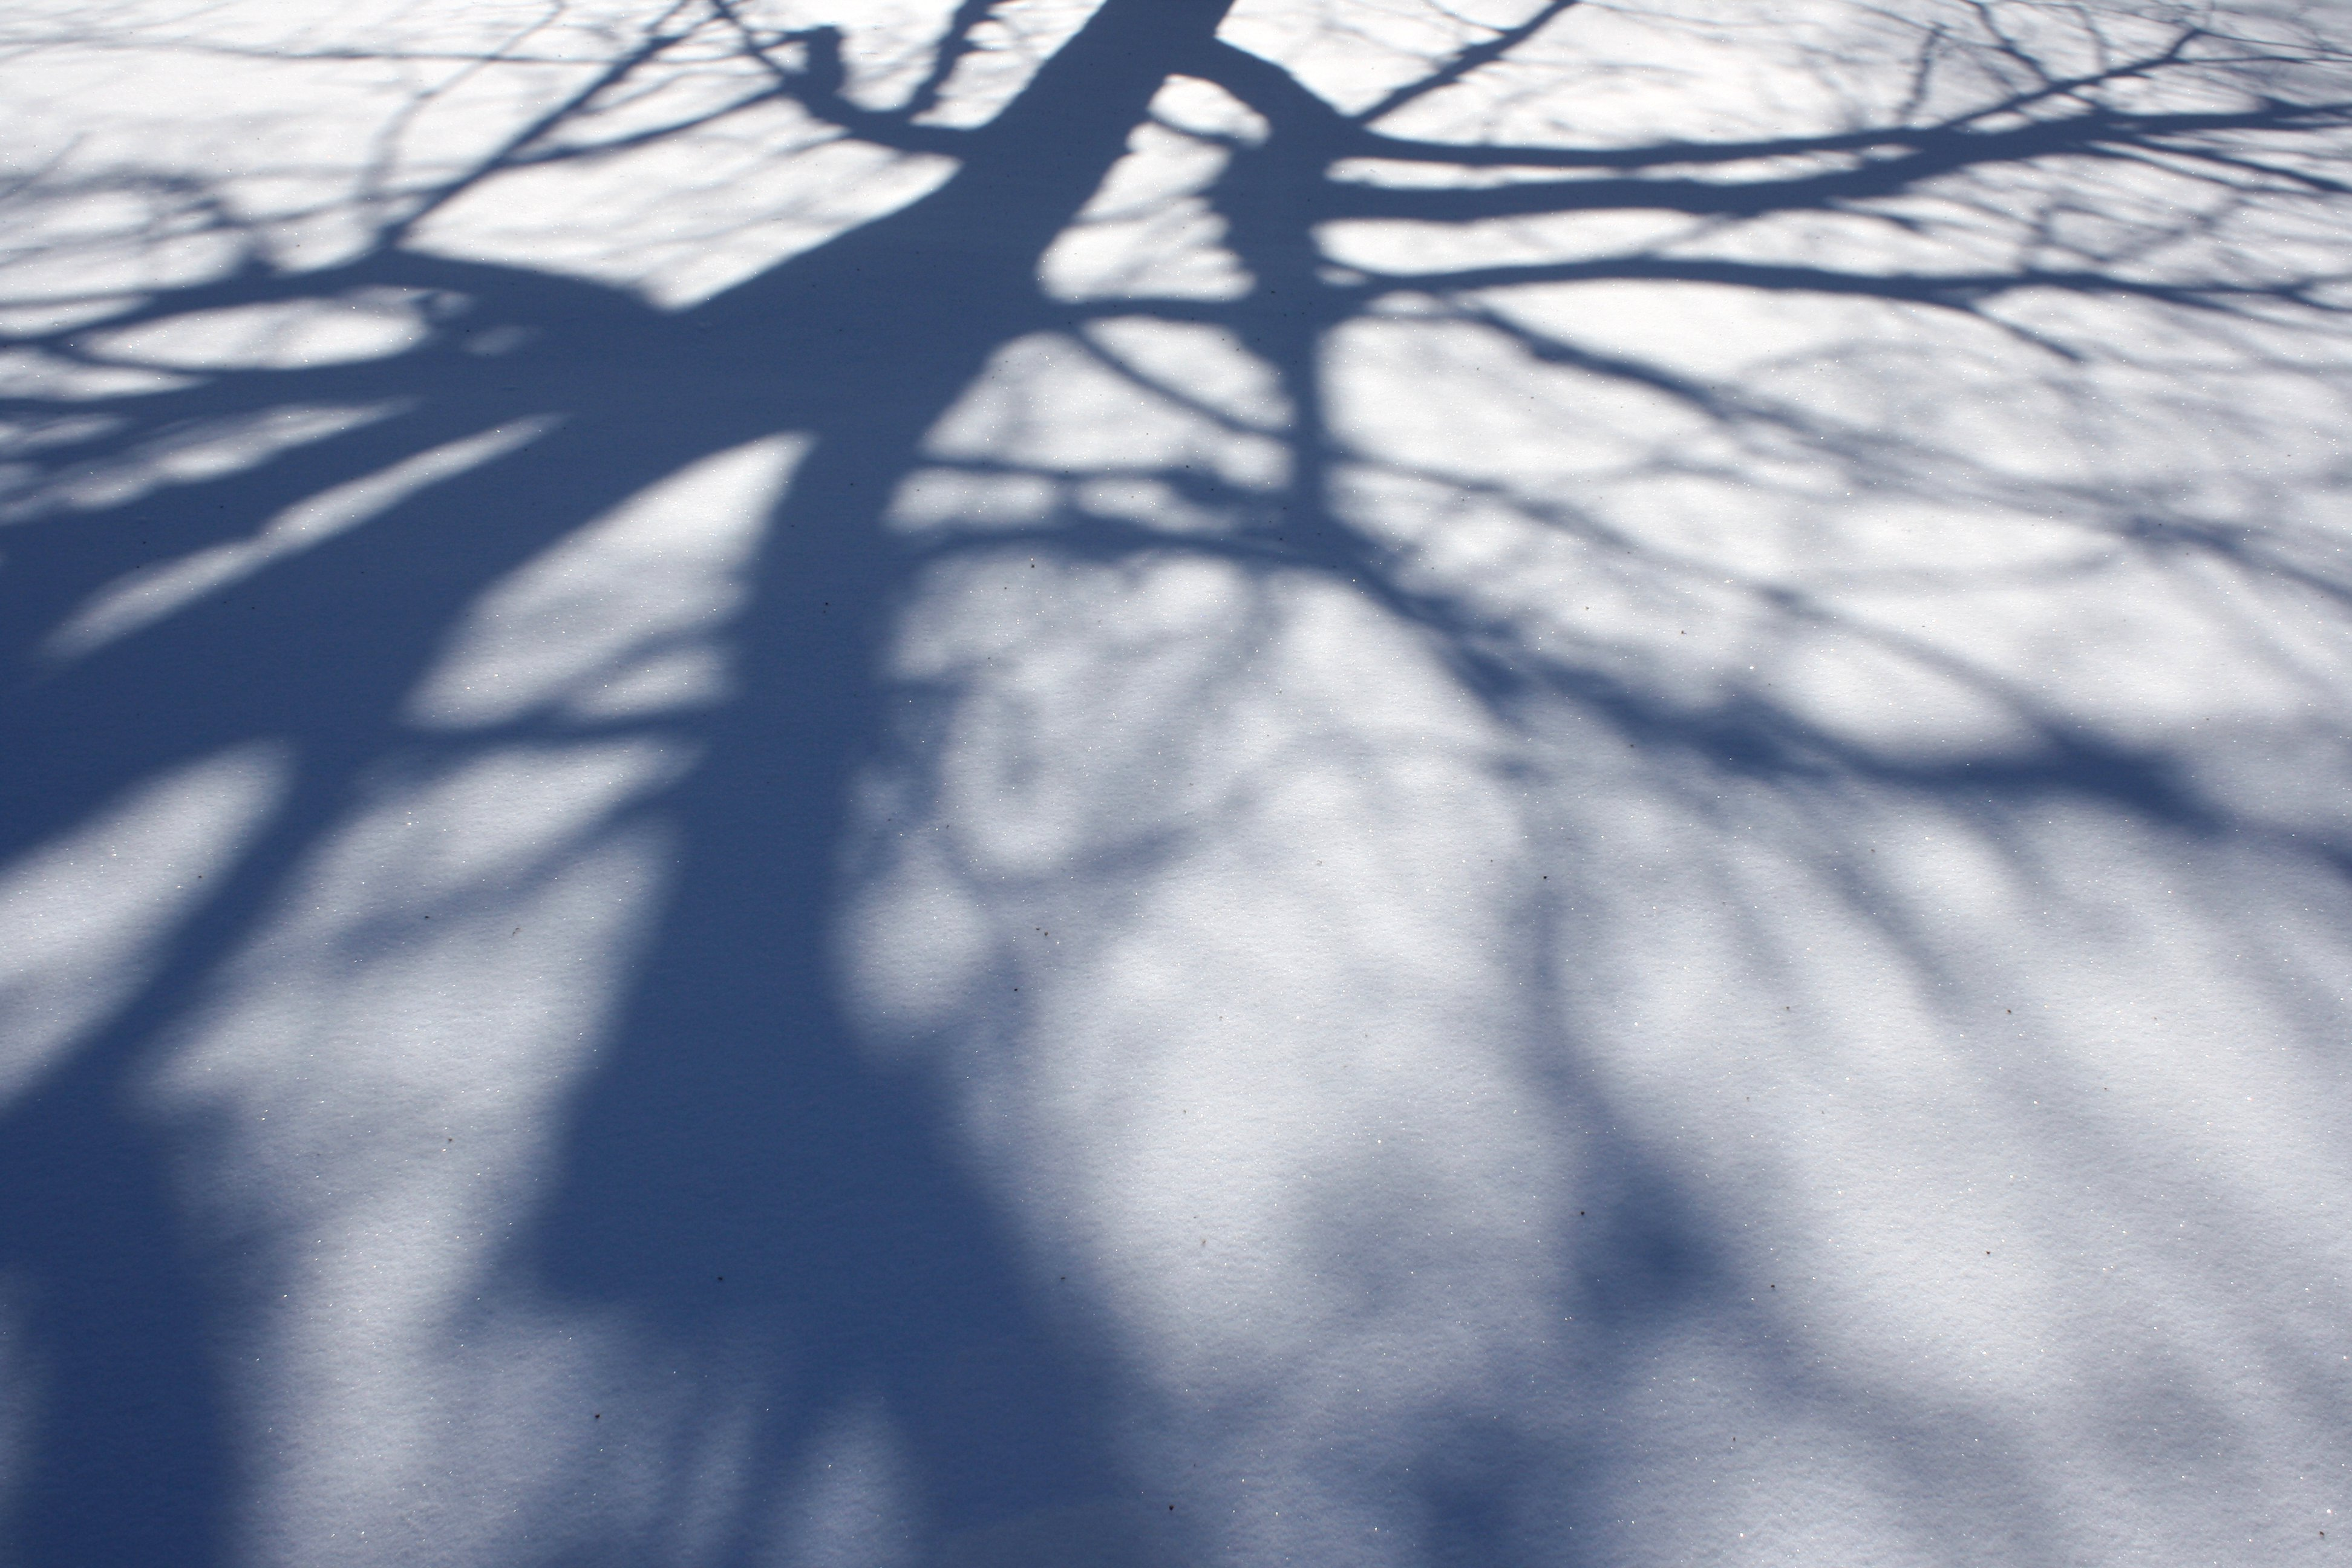
\includegraphics[width=14cm]{tree_shadow.jpg}
	\caption{The soft edges of a real shadow}
	\label{fig:shadow-soft-edge}
\end{figure}

\subsubsection{The Rendering Equation}
\cite{kajiya86therendering} presented a single integral equation which generalises a variety of rendering techniques. This equation has become known as "The Rendering Equation", the title of his 1986 paper. Solving it produces an accurate simulation of many effects, including soft shadows, depth of field, ambient occlusion, global illumination and motion blur. The physical basis to this equation is as an approximation to Maxwell's equation for electromagnetism. Solving this equation is the main challenge in realistic rendering~\parencite{dimov07numericalmethods}.

Ray tracing evaluates this integral at a single point, the point of the intersection of a ray with the scene, and as such, it is not a good approximation. For this reason, ray tracing is known as a point-sampling approach. A number of approaches have been developed to address this limitation, such as cone tracing, distributed ray tracing, and path tracing.

\begin{figure}
\centering
	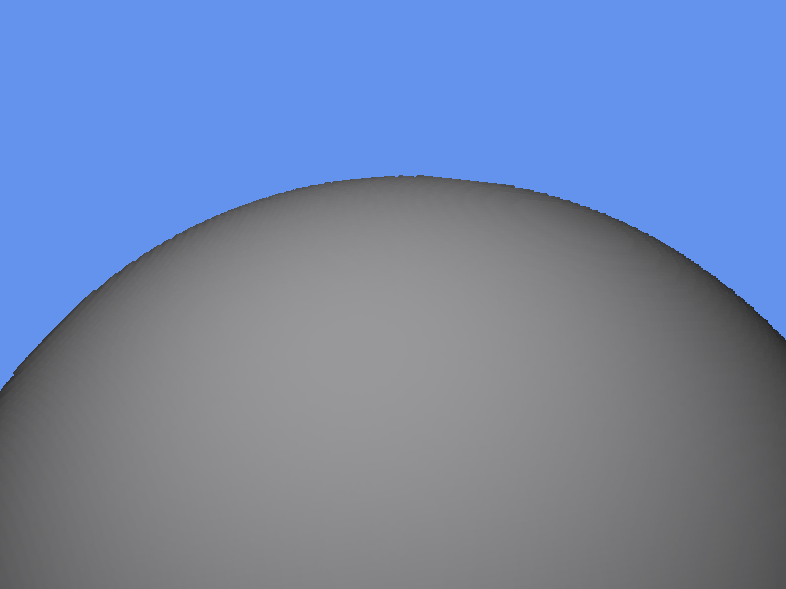
\includegraphics[width=14cm]{aliasing.png}
	\caption{The aliased edges caused by point sampling approaches}
	\label{fig:ray-tracing-aliases}
\end{figure}

\subsubsection{Cone tracing}
\citeauthor{amanatides84conetracing} presented a new method of ray tracing using cones rather than half-line rays in order to sample each pixel. The spread angle of the cone is chosen such that the radius of the cone's base is the size of the pixel according to the projection. The difficulty in using this method is the complexity of the intersection tests of a cone with the scene. \citeauthor{amanatides84conetracing} describes the necessary intersection calculations between a cone and various objects.

As cone tracing is no longer a point-sampling method, anti-aliasing is no longer required, and yet still only one sample per pixel is required. \citeauthor{amanatides84conetracing}' approach also allows for built in level of detail, soft shadows and blurred reflections. Given efficient intersection tests, this allows cone tracing to achieve similar performance to ray tracing with numerous advantages.

\subsubsection{Distributed ray tracing}
\cite{cook84distributed} also provides a solution to these problems with traditional ray tracing. By distributing the directions of the rays according to the analytic functions they sample, \citeauthor{cook84distributed}'s approach allows ray tracing to render fuzzy phenomena. By utilising this technique, \citeauthor{cook84distributed} enable ray tracing to produce blurred reflections, translucency and soft shadows, motion blur and depth of field.

The advantage of this approach over \citeauthor{amanatides84conetracing}' cone tracing approach is that the ray intersection calculations do not change, merely the ray directions are distributed~\parencite{cook84distributed}. Similarly to \cite{amanatides84conetracing}, the approach presented in this paper also does not require any more rays than vanilla ray tracing. The disadvantage to this approach is that the rays are still point-sampled, and therefore, anti-aliasing techniques are still required in order to reduce the effects of aliasing on the edges of objects.

\subsubsection{Path tracing}
\citeauthor{kajiya86therendering}'s own approach involves a Monte Carlo solution of the rendering equation. This Monte Carlo solution involves randomly distributing rays over the integral's domain, and then averaging them. This produces an extremely accurate and unbiased image, which naturally simulates many visual effects, including soft shadows, global illumination, and depth of field. Unfortunately, in order to get high quality images from this approach, a large number of rays must be traced in order to avoid very visible noisy artifacts.

Despite this, \citeauthor{bikker13brigade} have managed to get a path tracer running in real-time by utilising the persistent threads technique demonstrated by \cite{aila2009hpg}. This approach still displays noisy artifacts at first however, with the approximation improving over time as the camera is stationary and more samples are averaged. Despite this, the noise is still being improved, and with more computing power, the ability to average more samples per pixel faster will naturally reduce the amount of noise generated over time.